\documentclass[12pt]{beamer}
\usetheme{Hannover}
\usepackage{graphicx}
\usepackage{booktabs}
\usepackage[english]{babel}
\usepackage{kotex}
%\usepackage[pdfencoding=auto]{hyperref}
\hypersetup{pdfencoding=auto}
\usepackage{ulem}
\usepackage[per-mode=symbol]{siunitx}
\sisetup{inter-unit-product =$\cdot$}
\usepackage{verbatim}
\usepackage{listings}
\usepackage{tikz}
\setbeamertemplate{caption}[numbered]
\graphicspath{{images/}}
\lstset{language = [LaTeX]{TeX},
	basicstyle=\scriptsize\linespread{1}\ttfamily,
	tabsize=1,
	backgroundcolor=\color[gray]{0.9},
	showstringspaces=false
}
\title[\LaTeX - Day 2]{\LaTeX 입문 - Day 2}

\author{경기과학고 \TeX 사용자협회}
\institute[GSHSTeXSociety]{\url{latex.gs.hs.kr}}
\date{마지막 수정일 : \today}

\setbeamertemplate{navigation symbols}{}%to suppress navigation tools

\AtBeginSection[]{
	\begin{frame}
		\vfill
		\centering
		\begin{beamercolorbox}[sep=8pt,center,shadow=true,rounded=true]{title}
			\usebeamerfont{title}\insertsectionhead\par%
		\end{beamercolorbox}
		\vfill
	\end{frame}
}
\begin{document}

\begin{frame}
\titlepage % Print the title page as the first slide
\end{frame}

\begin{frame}{지난 시간에는}
	\begin{itemize}
		\item \TeX 소개, 설치, 문서 구조
		\item 워드프로세서 로서의 \TeX 기본사항
		\item 열거 환경
		\item 수식 입력 방법 및 SI 단위 사용법
		\item 문서 계층
		\item ToC, LoF, LoT
	\end{itemize}
	이번 시간에는 여러가지 그래픽 관련 요소를 배워 보겠다.
\end{frame}

\section{라벨링 및 상호 참조}
\begin{frame}{라벨링}
	수식\footnote{물론, \$ ... \$ 와 같은 단순한 mathmode 의 수식들은 불가능. equation* 환경과 같이 번호를 매기지 않는 수식도 마찬가지로 불가능하다.}, 그림, 표, 절 모두 라벨링이 가능하며, \textbf{번호가 자동으로 매겨진다.}
	
	라벨링을 할 때는 자신이 기억하기 쉬운 단어를 사용하면 된다. 단, 이 라벨이 수식, 그림, 표, 절인지 구분하지 위해서 라벨은 `eq\_', `fig\_', `tab\_', `sec\_' 와 같이 시작하는 것이 좋다.

	
\end{frame}

\begin{frame}{상호 참조}
	라벨을 참조하려면 \textbackslash ref\{라벨명\} 와 같이 사용하면 된다.
	등식의 경우 \textbackslash eqref\{...\} 를 사용해야 괄호가 쳐진 번호로 나타난다.
	
	예시는 아래와 같다. 코드 : \footnote{\url{http://pastebin.com/4jayE5X0}}
	\begin{figure}
		\centering
		\fbox{
\includegraphics[width=\textwidth]{test_crop_v2.pdf}}
	\end{figure}
\end{frame}
\begin{frame}{자동 조사 기능}
	한글로 논문을 작성할 경우 그림 1과..., 2와..., 와 같이 조사가 바뀌는 경우가 있다. 따라서 `\textbackslash 과', `\textbackslash 와' 와 같이 둘 중 아무 것이나 입력해 놓으면 자동으로 조사가 변경된다. 자동 조사 명령은 다음 12가지가 있다.
	\begin{center}
		\fbox{\small \textbackslash 이 \textbackslash 가, \textbackslash 을 \textbackslash 를, \textbackslash 와 \textbackslash 과, \textbackslash 로 \textbackslash 으로, \textbackslash 은 \textbackslash 는, \textbackslash 라 \textbackslash 이라}
	\end{center}
\end{frame}

\section{떠다니는 개체}

\subsection{그림 삽입}
\begin{frame}[fragile]{그림 삽입 : 기본적인 구조}
	\begin{center}
		\begin{scriptsize}
			\begin{verbatim}
			\begin{figure}[htbp]
			\centering
			\includegraphics[width=.3\textwidth]{example-image-a.jpg}
			\caption{Example Image a.}
			\label{fig_example_a}
			\end{figure}
			\end{verbatim}
		\end{scriptsize}
	\end{center}
	결과는 그림 \ref{fig_example_a}\와 같다.
	
	\begin{figure}[htbp]
		\centering
		\includegraphics[width=.3\textwidth]{example-image-a}
		\caption{Example Image a.}
		\label{fig_example_a}
	\end{figure}
\end{frame}
\begin{frame}[fragile]{그림 삽입 코드 설명}
	\begin{center}
		\begin{scriptsize}
			\begin{verbatim}
			\begin{figure}[htbp]
			\centering
			\includegraphics[width=.3\textwidth]{example-image-a.jpg}
			\caption{Example Image a.}
			\label{fig_example_a}
			\end{figure}
			\end{verbatim}
		\end{scriptsize}
	\end{center}
	\begin{itemize}
		\item htbp : 다음 슬라이드 참조
		\item \textbackslash centering : 그림의 중앙 정렬
		\item width=.3\textbackslash textwidth : 그림의 크기 = 본문 너비의 0.3배. width 외에도 height, scale을 사용 가능.
		\item example-image-a : 여기에 그림파일 이름을 넣으면 된다. 그림은 지정된 디렉토리\footnote{설정이 없을 경우 .tex 파일과 같은 디렉토리. \textbackslash graphicspath\{\{images/\}\} 와 같이 지정 가능하며, 훨씬 깔끔하다.}에 있으면 된다.
		\item 반드시 \textbf{caption 다음에 label}을 달아야 한다.
	\end{itemize}
\end{frame}
\begin{frame}{h,t,b,p 옵션}
	`\textbackslash begin\{figure\}' 바로 뒤의 대괄호에 등장하는 옵션에 대해 알아보자.
	\begin{table}
		\centering
		\begin{tabular}{|c|p{0.8\textwidth}|}
			\hline
			h & 개체를 코드의 위치(여기 : \textbf{h}ere)에 놓음 \\
			\hline
			t & 개체를 페이지의 맨 위쪽(\textbf{t}op)에 놓음 \\
			\hline
			b & 개체를 페이지의 맨 아래쪽(\textbf{b}ottom)에 놓음 \\
			\hline
			p & 개체를 특정 페이지(\textbf{p}age)에 놓음. 별다른 설정이 없으면 문서의 맨 뒤. \\
			\hline
			! & \LaTeX 에서 미리 설정해놓은 일부 서식을 무시하고(ex. 텍스트 여백) 놓음\\
			\hline
		\end{tabular}
	\end{table}
\end{frame}
\begin{frame}{h,t,b,p 옵션}
	보통의 워드프로세서를 사용하던 것처럼 하려면 단순히 h를 사용하면 된다. 하지만 때로는 h가 불가능하기 때문에, 이미지가 페이지 경계를 넘어간다든지 하는 일을 막으려면 htbp와 같이 차선책을 두어 주는 것이 좋다. tpbh 등으로 설정해도 htbp 순으로 적용된다.
	
	또한, 대부분의 학술지는 두 단으로 나누어진 양식을 채택하는데, 이 경우 그림을 페이지의 중간에 놓는 것보다는 맨 위에 두고, 맨 위에 둘 수 없다면 맨 아래에 두는 것이 좋다. 다음 두 페이지의 예시를 보자.
\end{frame}
\begin{frame}{품위 있는 그림 및 표 배치}
	\begin{figure}[h]
		\centering
		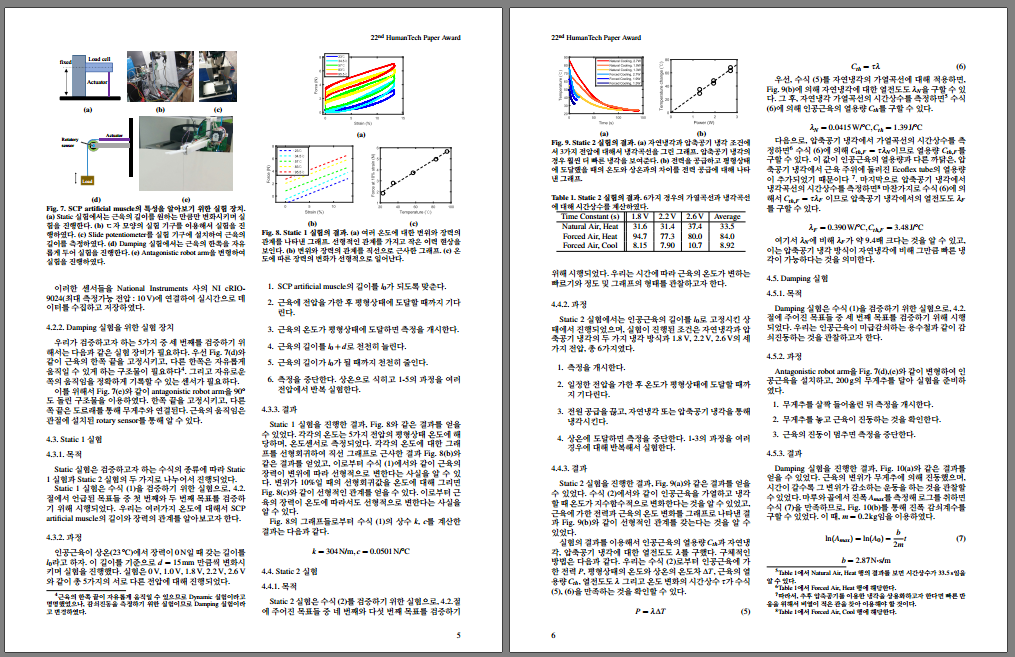
\includegraphics[width=.9\textwidth]{right_fig.png}
	\end{figure}
	\footnote{출처 : 김형주, 박승원, ``SCP Artificial Muscle로 작동하는 Antagonistic Robot Arm의 Feedback 제어''(2015)}
\end{frame}
\begin{frame}{올바르지 못하게 했을 경우}
	
	{\small (같은 논문에서 [t] 옵션을 모두 [h] 로 바꾼 결과이다.)}
	\begin{figure}[h]
		\centering
		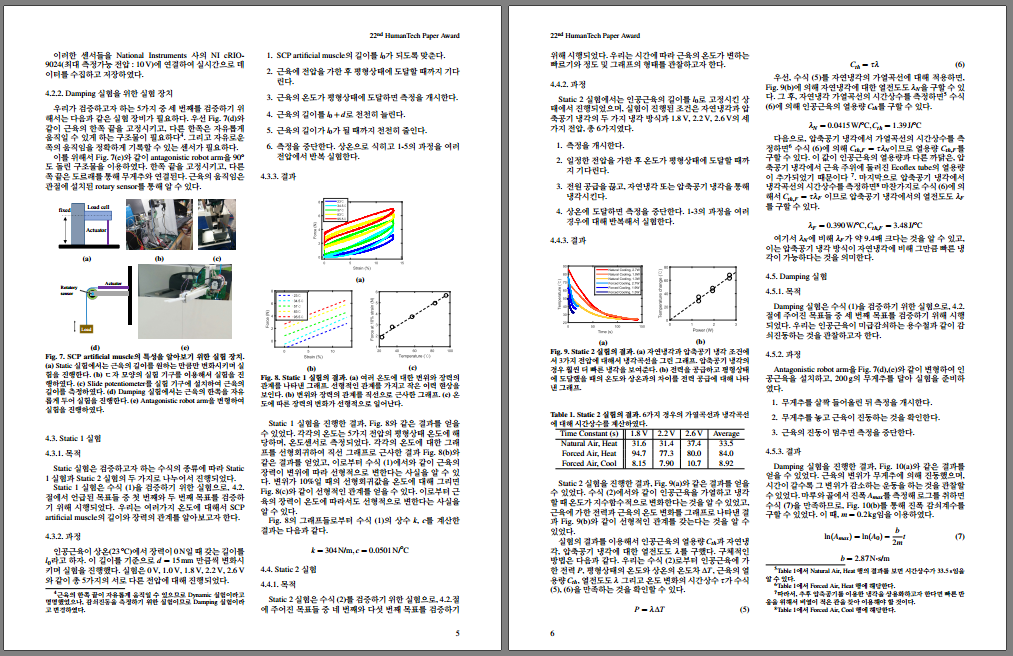
\includegraphics[width=.9\textwidth]{wrong_fig_v2.png}
	\end{figure}
\end{frame}
\begin{frame}{정확한 위치에 놓기}
	다만 때에 따라서는 그림을 정확한 위치에 놓아야 할 때가 있다.
	
	그럴 때는 `float' package의 H 옵션을 사용하자. figure 환경에서 htbp 대신 H를 사용하면 된다.
\end{frame}
\begin{frame}{그림의 유형}
	삽입할 그림의 유형에 대해 적합한 이미지 형식은 다음과 같다.
	\begin{itemize}
		\item 사진 : jpg 또는 jpeg 파일
		\item 그래프 : pdf 또는 eps (벡터 이미지)
		\item 기하적 그림 : png로 캡처 혹은 벡터 이미지
		\item 일러스트 : pdf
	\end{itemize}
	\begin{footnotesize}
		기하적 그림의 경우, GeoGebra에서는 export to tikz 가 되며, standalone class를 이용해 벡터 이미지로 뽑아낼 수 있다. 필요하면 찾아보시길.
		
		일러스트의 경우 보통 PowerPoint로 만든다. `pdf로 내보내기' 기능을 이용하여 .pdf 형식의 벡터 이미지를 얻을 수 있다.
		
		pdf 이미지의 여백이 심할 경우 online pdfcrop 을 찾아보라.
	\end{footnotesize}
\end{frame}
\begin{frame}[fragile]{Subfigure}
	예시 및 코드\footnote{\url{http://pastebin.com/fUSHv8FK}} : 
	\begin{figure}
		\centering
		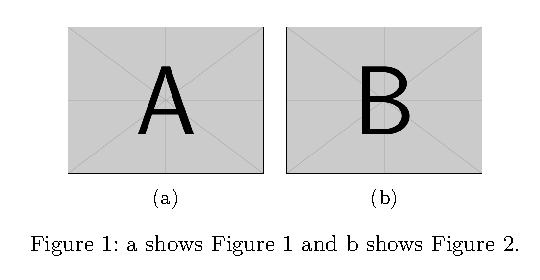
\includegraphics[width=.8\textwidth]{subfigure.pdf}
	\end{figure}
\end{frame}
\subsection{표 삽입}
\begin{frame}[fragile]{표 삽입}
	그림 삽입을 배우고 나면 표는 비교적 간단하다.
	
	인터넷에 latex table generator가 있으니, 이것을 사용하는 것도 꽤 편리하다고 한다. 
	하지만 일단은 설명해 보겠다. 표의 기본적인 구조는 다음과 같다.
	\begin{columns}
		\begin{column}{.4\textwidth}
			\begin{center}
				\begin{scriptsize}
					\begin{verbatim}
					\begin{table}[htbp]
					\centering
					\begin{tabular}{|l|c|r|}
					\hline
					학번&이름&특징\\
					\hline
					\hline
					14041&홍길동&호부호형 못함.\\
					\hline
					14004&전우치&도술에 재능.\\
					\hline
					\end{tabular}
					\end{table}
					\end{verbatim}
				\end{scriptsize}
			\end{center}
		\end{column}
		\begin{column}{.5\textwidth}
			\begin{scriptsize}
				\begin{table}[htbp]
					\centering
					\begin{tabular}{|l|c|r|}
						\hline
						학번&이름&특징\\
						\hline
						\hline
						14200&홍길동&호부호형 못함.\\
						\hline
						14300&전우치&도술에 재능.\\
						\hline
					\end{tabular}
				\end{table}
			\end{scriptsize}
		\end{column}
	\end{columns}
\end{frame}
\begin{frame}{표 작성하기}
	\begin{table}
		\centering
		\begin{tabular}{|c|c|}
			\hline
			l & 좌측 정렬 열 \\
			\hline
			c & 중앙 정렬 열 \\
			\hline
			r & 우측 정렬 열 \\
			\hline
			p\{`width'\} & 폭이 지정된 열. 상측 정렬됨. \\
			\hline
			\textbar & 수직 선(여러 개 사용가능) \\
			\hline
			\& & 열 구분 기호 \\
			\hline
			\textbackslash\textbackslash & 개행 \\
			\hline
			\textbackslash hline & 수평 선(여러 개 사용가능) \\
			\hline
			\textbackslash cline\{i-j\} & i열부터 j열까지의 수평 선 \\
			\hline
		\end{tabular}
	\end{table}
\end{frame}
\begin{frame}{표 예시}
	조금(?) 어려운 표의 예시이다. 보면서 공부하면 도움이 될 것이다.
	코드 : \footnote{\url{http://pastebin.com/1A8L4HjG}}
	\begin{figure}
		\centering
		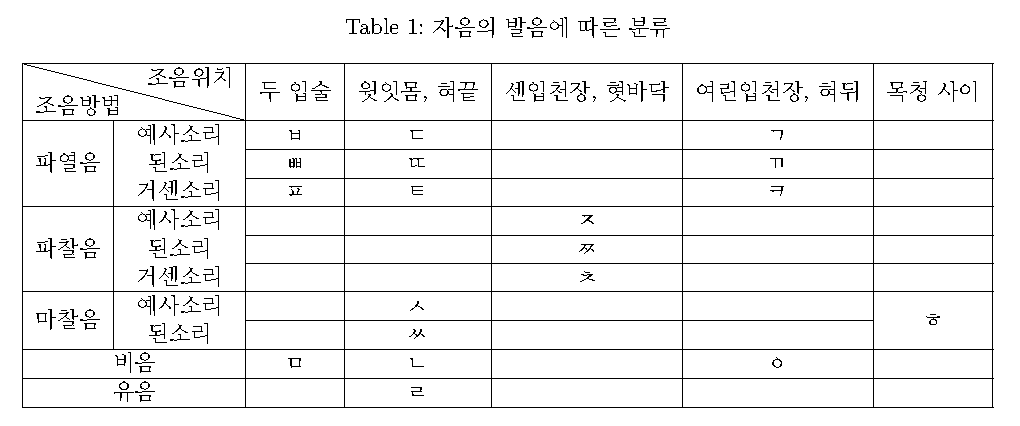
\includegraphics[width=\textwidth]{table_adv.pdf}
	\end{figure}
\end{frame}
\section{tikz}
\begin{frame}[fragile]{패키지}
	tikz를 사용하기 위해서는
	\begin{lstlisting}
	\usepackage{tikz}
	\end{lstlisting}
	로 tikz 패키지를 추가해야 한다
	\vfill
	\begin{lstlisting}
	\usetikzlibrary{}
	\end{lstlisting}
	로 라이브러리를 추가할 수도 있다
	
	유용한 라이브러리로 tkz-euclide 등이 있다
\end{frame}

\begin{frame}[fragile]{사용 환경}
	tikz로 그림을 그리는 방법은 다음 두 가지가 있다
	\vfill
	\begin{lstlisting}
	\begin{tikzpicture}[option]
	(tikz command)
	\end{tikzpicture}
	\end{lstlisting}
	\vfill
	\begin{lstlisting}
	\tikz[option]{(tikz command)}
	\end{lstlisting}
	\vfill
	tikz 명령어 맨 뒤에는 반드시 세미콜론(;)을 붙여야 한다
\end{frame}

\begin{frame}{위치}
	tikz는 데카르트 좌표계와 극좌표계를 사용한다
	\vfill
	오른쪽으로 가면 x좌표가 증가하고
	
	위쪽으로 가면 y좌표가 증가한다
	\vfill
	화면의 중심은 (0,0)이 아니고 내가 그린 그림이 알맞은 위치에 오도록 알아서 맞춰지므로 점들의 간격만 신경쓰면 된다
\end{frame}


\subsection{점}

\begin{frame}{\secname}{표기}
	점은 \((x,y)\) 또는 \((\theta:r)\) 로 나타낸다
	
	\vfill
	(10cm,2pt)같이 길이의 단위를 쓸 수 있다
	
	단위를 쓰지 않으면 기본으로 cm가 적용된다
\end{frame}

\begin{frame}[fragile]{\secname}{node}
	다음과 같이 좌표를 지정할 수 있다
	\begin{lstlisting}
	\node[option](name) at (coordinate){text};
	\coordinate[option](name) at (coordinate);
	\end{lstlisting}
	\vfill
	점은 화면에 나타나지 않는다
	
	나타나는 것은 text 뿐이다
	\vfill
	점의 이름은 생략할 수 있다
	
\end{frame}

\begin{frame}[fragile]{\secname}{path}
	path를 사용해 여러개의 점을 한꺼번에 지정할 수 있다
	
	\begin{lstlisting}
	\path(coordinate) node[options](name){text}
	... (coordinate) node[options](name){text};
	\end{lstlisting}
	\vfill
	원하는 만큼 node나 coordinate로 점을 지정하면 된다
	
\end{frame}

\begin{frame}[fragile]{\secname}{example}
	\begin{lstlisting}
	\node (a) at (0:3){This is a};
	\coordinate (b) at (0,10);
	\path(0,0) node(x) {X}
	(3,3) node(y) {Y};
	\end{lstlisting}
	
	\begin{center}
		\begin{tikzpicture}
		\node (a) at (0:3){This is A};
		\coordinate (b) at (0,3);
		\path (0,0) node(x) {X}
		(3,3) node(y) {Y};
		\end{tikzpicture}
	\end{center}
	
\end{frame}


\subsection{선}

\subsubsection{선분}
\begin{frame}[fragile]{\secname}{\subsecname}
	다음과 같이 여러 선분을 이어서 그릴 수 있다
	\begin{lstlisting}
	\draw[option](0,0) -- (1,1) -- (3,0);
	\end{lstlisting}
	
	\tikz{\draw[thick] (0,0) -- (1,1) -- (3,0);}
	
	\vfill
	앞에서 점의 이름을 지어주었다면 좌표 대신 이름을 쓸 수도 있다
\end{frame}
\begin{frame}[fragile]{\secname}{\subsecname}
	두 점을 그냥 잇지 않고 택시거리로 연결할 수도 있다
	\begin{lstlisting}
	\draw(0,0) |- (1,1);
	\draw(2,0) -| (3,1);
	\end{lstlisting}
	
	\tikz{\draw[thick] (0,0) |- (1,1);\draw[thick] (2,0) -| (3,1);}
	
	\vfill
	이런 것도 가능하다
	\begin{lstlisting}
	\draw(0,0 |- 1,1) -- (2,0 -| 3,1);
	\end{lstlisting}
	\tikz{\draw[thick] (0,0 |- 1,1) -- (2,0 -| 3,1);}
	
\end{frame}

\subsubsection{곡선}
\begin{frame}[fragile]{\secname}{\subsecname}
	베지에 곡선\footnote{\url{https://en.wikipedia.org/wiki/B\%C3\%A9zier_curve}\\}을 다음과 같이 만들 수 있다
	\begin{lstlisting}
	\draw(0,0) .. controls(1,1) .. (3,0); 
	\draw(4,0) .. controls(5,1) and (6,1) .. (7,0);
	\end{lstlisting}
	\tikz{\draw (0,0) .. controls (1,1) .. (3,0);\draw (4,0) .. controls (5,1) and (6,1) .. (7,0);\draw[dashed] (0,0) -- (1,1) -- (3,0);\draw[dashed] (4,0) -- (5,1) -- (6,1) -- (7,0);}
	
	\vfill
	{\footnotesize (그냥 점들을 이은 선분들을 뒤에 점선으로 표시해 보았다)}
\end{frame}

\subsubsection{화살표}
\begin{frame}[fragile]{\secname}{\subsecname}
	화살표를 만드는 것은 매우 간단하다
	\begin{lstlisting}
	\draw[->,thick](0,0) -- (1,1) -- (3,0);
	\end{lstlisting}
	
	\tikz{\draw[thick,->] (0,0) -- (1,1) -- (3,0);}
	
	\begin{lstlisting}
	\draw[<->,dashed](0,0) .. controls(1,1) .. (3,0);
	\end{lstlisting}
	
	\tikz{\draw[<->,dashed] (0,0) .. controls (1,1) .. (3,0);}
	
\end{frame}

\subsection{도형}
\subsubsection{다각형}
\begin{frame}[fragile]{\secname}{\subsecname}
	점들을 이어 도형을 만들어주면 된다
	
	다시 첫번째 점을 쓰지 않고 cycle이라 쓸 수 있다
	\begin{lstlisting}
	\draw[thick](0,0) -- (1,1) -- (3,0) -- cycle;
	\end{lstlisting}
	
	\tikz{\draw[thick] (0,0) -- (1,1) -- (3,0) -- cycle;}
	
	색을 칠하고 싶으면 filldraw를 사용한다
	
	\begin{lstlisting}
	\filldraw[brown](0,0) -- (1,1) -- (3,0) -- cycle;
	\end{lstlisting}
	
	\tikz{\filldraw[brown] (0,0) -- (1,1) -- (3,0) -- cycle;}
	
\end{frame}
\subsubsection{원}
\begin{frame}[fragile]{\secname}{\subsecname}
	원의 중심 좌표를 쓴 뒤에 반지름을 써준다
	
	\begin{lstlisting}
	\draw(0,0) circle[radius=5mm];
	\end{lstlisting}
	
	\tikz{\draw (0,0) circle[radius=1];}
	
	타원은 장축과 단축의 길이를 써준다
	\begin{lstlisting}
	\draw(0,0) circle[x radius = 2, y radius = 1];
	\end{lstlisting}
	
	\tikz{\draw (0,0) circle[x radius = 2, y radius = 1];}
\end{frame}

\subsubsection{호}
\begin{frame}[fragile]{\secname}{\subsecname}
	호의 시작 좌표를 쓴 뒤에 각도 범위와 반지름을 써준다	
	\begin{lstlisting}
	\draw(8mm,0) arc(0:270:8mm);
	\filldraw(0,0) circle[radius=1pt] node[above] {O}
	\end{lstlisting}
	
	\tikz{\draw (8mm,0) arc (0:270:8mm);\filldraw (0,0) circle[radius=1pt] node[above] {O}}
	\begin{lstlisting}
	\filldraw(0,0) -- (12mm,0mm) arc(0:30:12mm) -- cycle;
	\end{lstlisting}
	
	\tikz{\filldraw (0,0) -- (12mm,0) arc (0:30:12mm) -- cycle;}
\end{frame}


\subsection{좌표 평면}
\subsubsection{좌표계}
\begin{frame}[fragile]{\secname}{\subsecname}
	좌표계를 다음과 같이 그릴 수 있다
	\begin{lstlisting}
	\draw[step=5mm, gray, thin](-1.2,-1.2) grid (1.2,1.2);
	\draw[->,thick](-1.25,0) -- (1.25,0);
	\draw[->,thick](0,-1.25) -- (0,1.25);
	\end{lstlisting}
	
	\tikz{\draw[step=5mm, gray, thin] (-1.2,-1.2) grid (1.2,1.2);\draw[->,thick] (-1.25,0) -- (1.25,0);\draw[->,thick] (0,-1.25) -- (0,1.25);}
	\vfill
	step으로 지정한 간격의 배수 위치에 격자가 생긴다
\end{frame}

\subsubsection{함수}
\begin{frame}[fragile]{\secname}{\subsecname}
	정의역을 정해주고 함수를 쓰면 점을 찍어준다
	
	샘플 수를 늘려주면 더 매끄럽게 된다
	\begin{lstlisting}
	\draw[step=5mm, gray, thin](-1.2,-1.2) grid (1.2,1.2);
	\draw[domain=-1:1,samplse=50] plot(\x,{sin(pi*\x r)});
	\end{lstlisting}
	
	\tikz{\draw[step=5mm, gray, thin](-1.2,-1.2) grid (1.2,1.2);\draw[domain=-1:1,samples=50] plot(\x,{sin(pi*\x r)});}
	\vfill
	함수를 중괄호로 감싸주어야 한다
	
	(x뒤의 r은 radian을 쓰라는 뜻이다)
\end{frame}
\end{document}